%% LaTeX2e class for student theses
%% sections/main/6_implementation.tex
%%
%% Karlsruhe University of Applied Sciences
%% Faculty of  Computer Science and Business Information Systems
%%
%% --------------------------------------------------------
%% | Derived from sdqthesis by Erik Burger burger@kit.edu |
%% --------------------------------------------------------

\chapter{Implementation}
\label{ch:Implementation}

\section{Resources}
\label{ch:Design:sec:Resources}

In case of a reservation system, the basic resource this system has to handle is defined as a \verb|reservation|. The according  endpoints exposed by the application for providing the functionalities to interact with the resource and required in the frontend parts of the application are listed below.

\begingroup
\setlength{\tabcolsep}{10pt} % Default value: 6pt
\renewcommand{\arraystretch}{1.5} % Default value: 1
\begin{table}[!ht]
\centering
\caption{Provided \acrshort{rest} endpoints }
    \begin{tabular}{l|c|m{5cm}}
    Resource Identifier & HTTP Method & Functionality \\ \hline
    \multicolumn{3}{c}{\verb"/reservations"} \\ \hline
    \verb|/| & \verb|GET|, \verb|POST|, \verb|DELETE| & Get a list of reservations \\
    \verb|/{id}| & \verb|GET|, \verb|PUT|, \verb|DELETE| & Read, update and delete operation for a specific reservation \\
    \verb|/{id}/cancel| & \verb|PUT| & Cancel a existing reservation by its ID \\
    \verb|/action/export| & \verb|GET| & Export existing reservations \\
    \multicolumn{3}{c}{\verb"/charging-stations"} \\ \hline
    \verb|/{id}/reserve/now| & \verb|PUT| & Reserve a connector at a \acrshort{cs} with ID \\
    \verb|/{id}/reservation/cancel| & \verb|PUT| & Cancel a reservation on a connector at a \acrshort{cs} with ID \\
    \verb|/reservation/availability| & \verb|GET| & Get reservable \acrshortpl{cs} for a specific time range 
    \end{tabular}
\label{tab:rest-endpoints}
\end{table}
\endgroup

\section{Implemented Use Cases}
\label{ch:Implementation:sec:Implemented Use Cases}

Afterwards, the implemented use cases will be described in details.

\subsection{Create Reservation}
\label{ch:Implementation:sec:Implemented Use Cases:ssec:Create Reservation}

\begin{figure}[!ht]
    \centering
    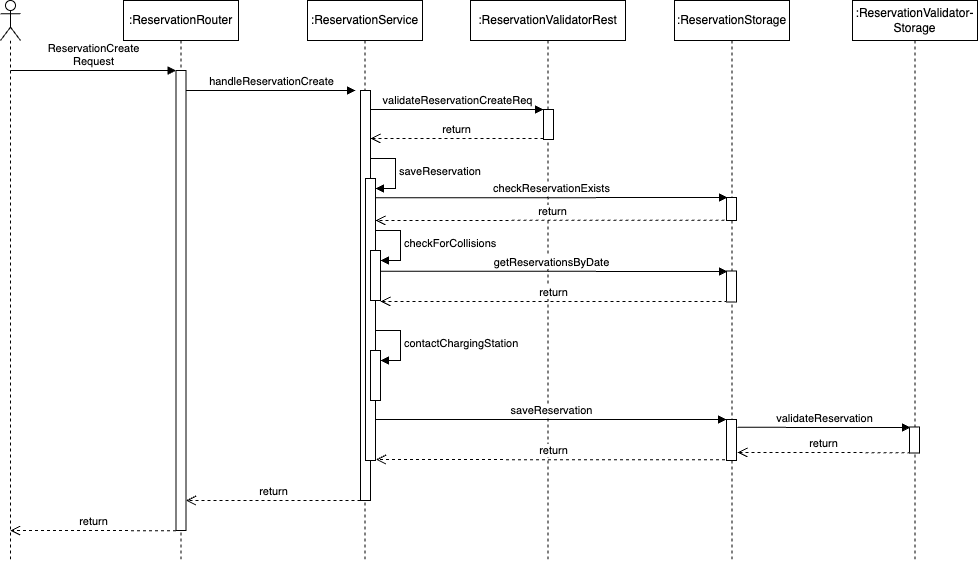
\includegraphics[scale=0.4]{resources/images/main/6_implementation/processes/ReservationCreate.png}
    \caption{Flow of information through the single components of the backend service}
    \label{fig:create-reservation-seq-flow}
\end{figure}

\subsection{Update Reservation}
\label{ch:Implementation:sec:Implemented Use Cases:ssec:Update Reservation}


\begin{figure}[!ht]
    \centering
    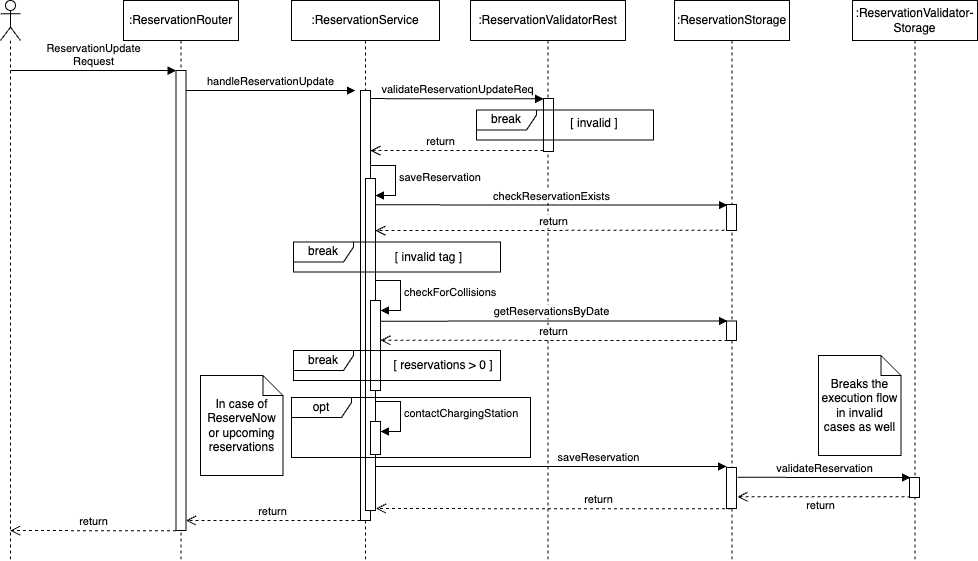
\includegraphics[scale=0.4]{resources/images/main/6_implementation/processes/ReservationUpdate.png}
    \caption{Flow of information through the single components of the backend service}
    \label{fig:update-reservation-seq-flow}
\end{figure}

\subsection{Delete Reservation}
\label{ch:Implementation:sec:Implemented Use Cases:ssec:Delete Reservation}

\begin{figure}[!ht]
    \centering
    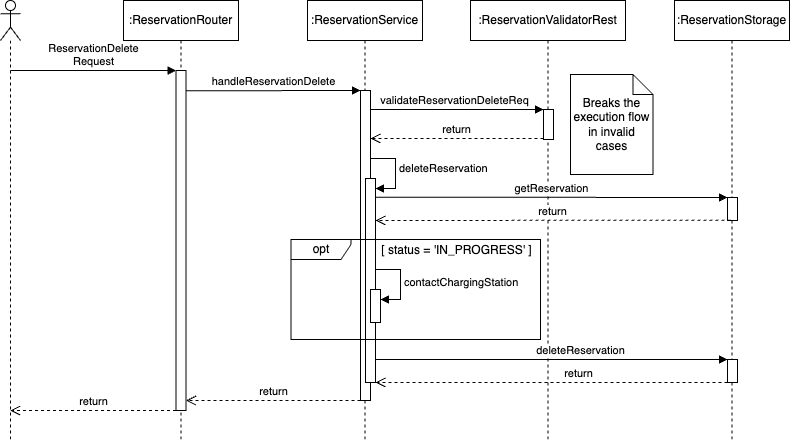
\includegraphics[scale=0.4]{resources/images/main/6_implementation/processes/ReservationDelete.png}
    \caption{Flow of information through the single components of the backend service}
    \label{fig:delete-reservation-seq-flow}
\end{figure}

\subsection{Cancel Reservation}
\label{ch:Implementation:sec:Implemented Use Cases:ssec:Cancel Reservation}


\begin{figure}[!ht]
    \centering
    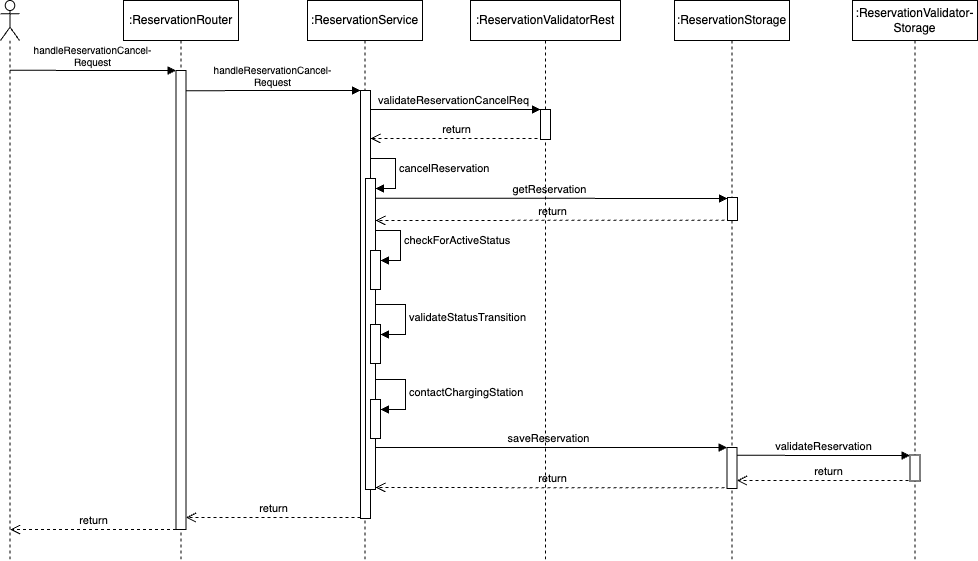
\includegraphics[scale=0.4]{resources/images/main/6_implementation/processes/ReservationCancel.png}
    \caption{Flow of information through the single components of the backend service}
    \label{fig:cancel-reservation-seq-flow}
\end{figure}

\subsection{Schedule Reservation}
\label{ch:Implementation:sec:Implemented Use Cases:ssec:Schedule Reservation}

\dots

% \begin{figure}[!ht]
%     \centering
%     \includegraphics[scale=0.4]{resources/images/main/6_implementation/processes/scheduler/SynchronizeReservation.png}
%     \caption{Flow of information through the single components of the backend service}
%     \label{fig:schedule-reservation-flow}
% \end{figure}

\subsection{Expire Reservation}
\label{ch:Implementation:sec:Implemented Use Cases:ssec:Expire Reservation}

\dots

\subsection{Free reserved connectors}
\label{ch:Implementation:sec:Implemented Use Cases:ssec:Free reserved connectors}

\dots

% \begin{figure}[!ht]
%     \centering
%     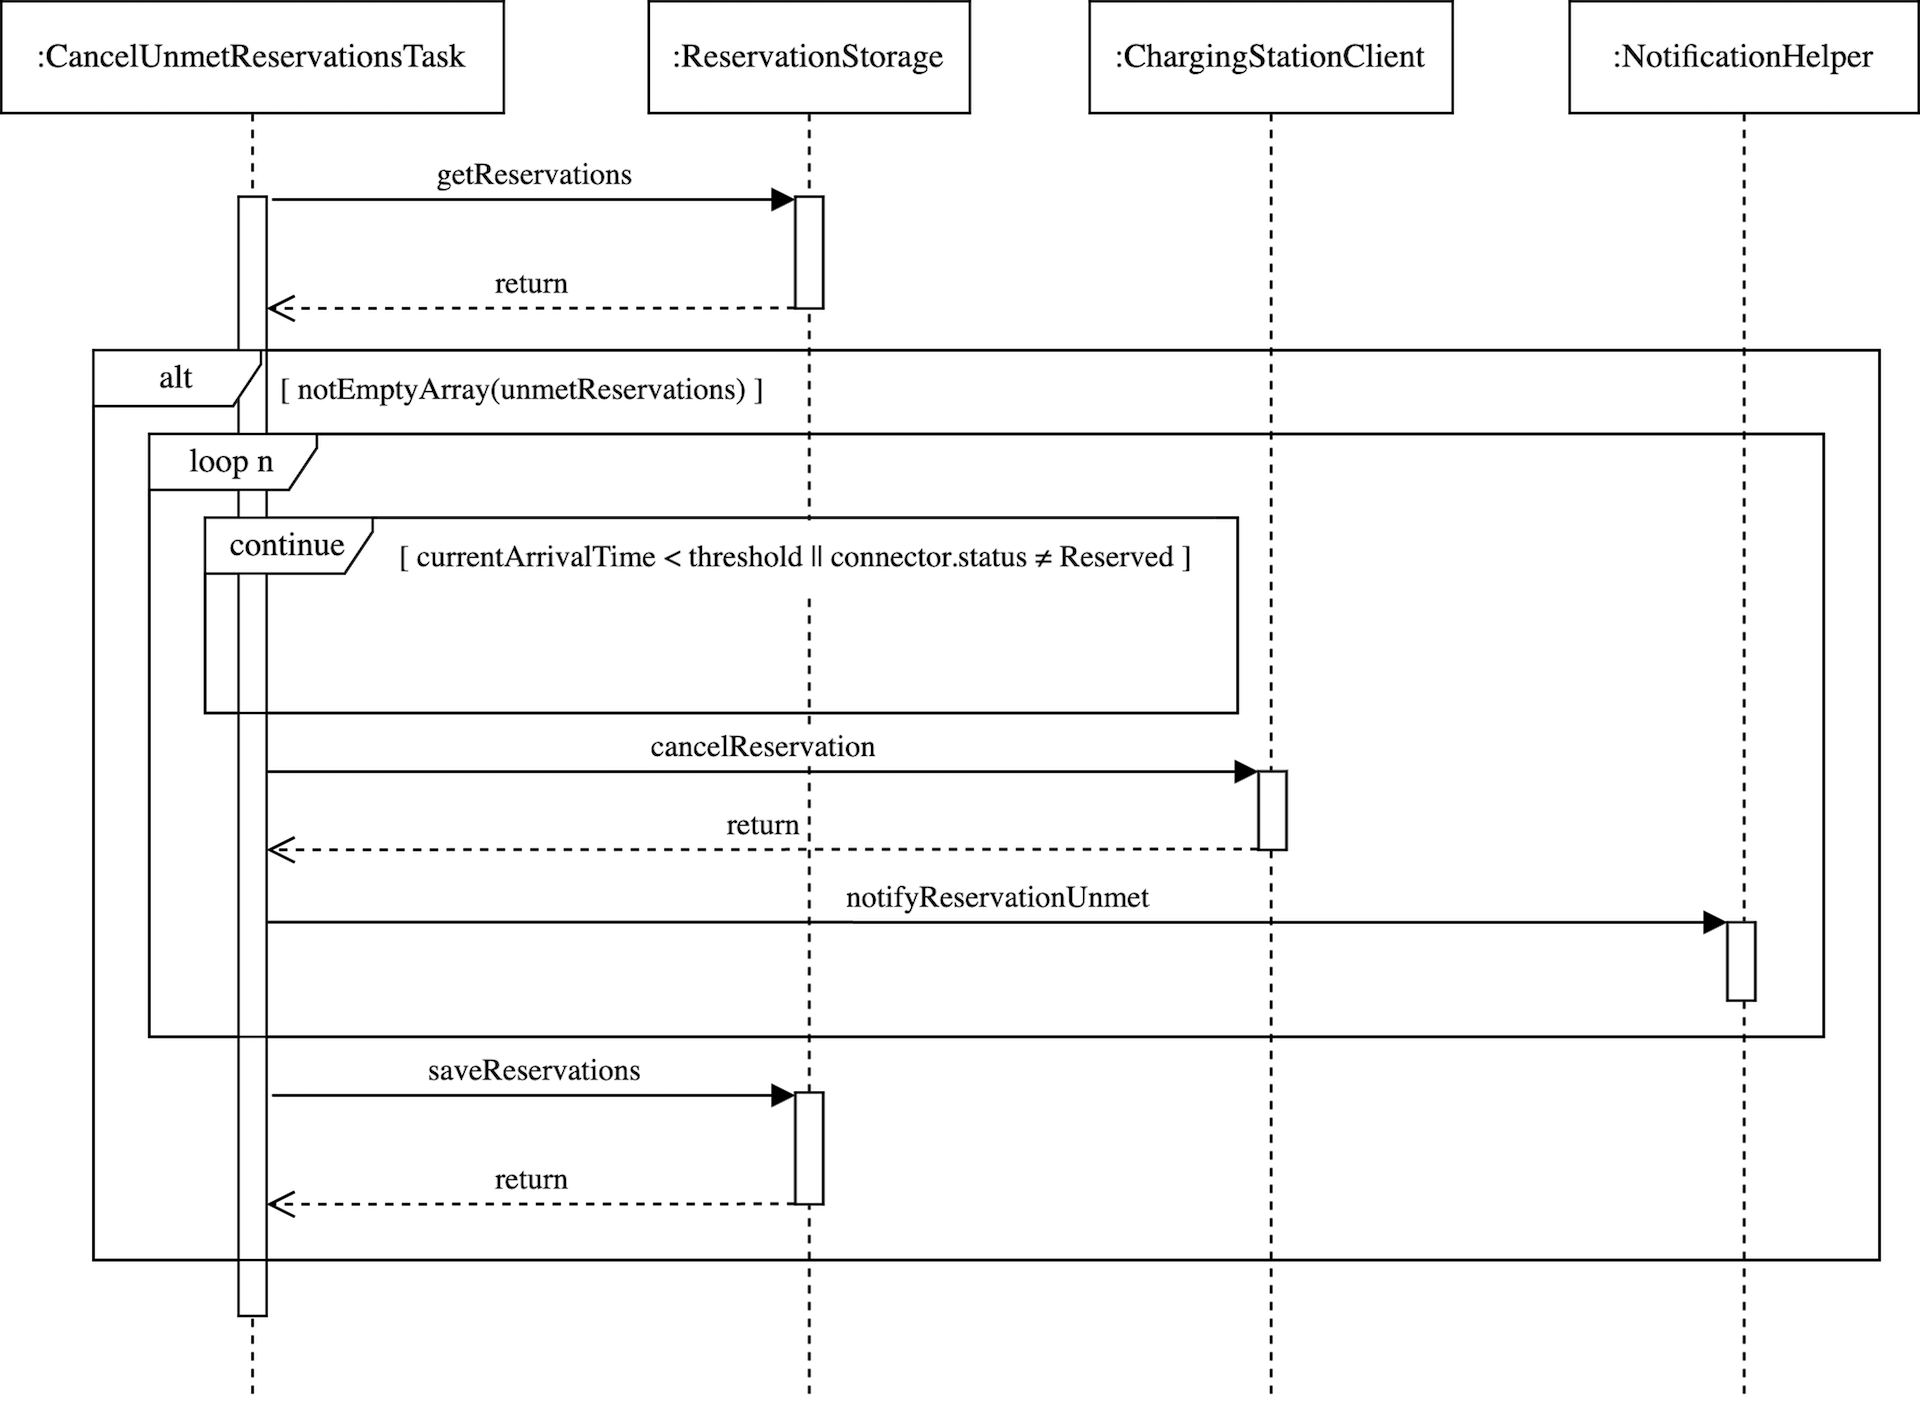
\includegraphics[scale=0.4]{resources/images/main/6_implementation/processes/scheduler/CancelUnmetReservation.png}
%     \caption{Flow of information through the single components of the backend service}
%     \label{fig:free-connector-flow}
% \end{figure}